% #############################################################################
% This is Chapter 2
% !TEX root = ../main.tex
% #############################################################################
% Change the Name of the Chapter i the following line
\fancychapter{Related work and Theoretical Background}
\cleardoublepage
% The following line allows to ref this chapter
\label{chap:back}

This chapter presents some background and related work. The chapter is divided into two main sections: \ref{sefs} \nameref{sefs} and \ref{sets} \nameref{sets}. Section \ref{sefs}  provides some literature review about \acp{EFS}, with a focus on the most effective methodologies for designing \ac{EFS}, followed by a review of some research and commercial projects. Section \ref{sets} presents instead some important concepts around blockchain technology, the rationale behind the use of blockchain in the energy sector, and some existing \ac{ET} research and commercial projects that leverage blockchain technology.


% #############################################################################
\section{Eco Feedback Systems} \label{sefs}

As mentioned before, \ac{EF} is defined as a technology that "provides feedback on individual or group behaviors with a goal of reducing environmental impact" \cite{Froehlich2010}. Its effectiveness has been demonstrated by over 40 years of research in multiple fields, nevertheless, designing an effective \ac{EFS} is everything but simple. Indeed, it requires a deep understanding of people latent motivations for sustainable behavior.


In the following pages, a brief (and likely not comprehensive) review of the main aspects to consider when designing an \ac{EFS} is presented.


\subsection{Models of pro-environmental behavior}

Understanding the motivations that lead people to act environmentally is a prerequisite when talking about \acp{EFS}. According to the literature on \ac{EF}, the two main models of human behavior to consider in this case are Rational Choice Model and Norm-activation model \cite{Froehlich2010}.


The Rational Choice Model assumes that human behavior is, like in game theory, based on the evaluation of expected utility. Basically, according to this model, people do things only if the result of their actions brings some reward. This reward may be monetary or not, like comfort, convenience, etc.


The second model implies that moral or personal norms are direct determinants of social behavior, in other words, if a person is aware of the negative impact of his/her behavior, he/she will feel the moral obligation to modify such behavior.


Selecting one model or the other depends on the user type we are designing for and, consequently, it strongly influences the type of feedback information to be presented. For example, a design based on the rational choice model should show savings in the electricity bill, while presenting the impact of the user behaviors on the Amazon forest would be more consistent with a design based on the norm-activation model.

\subsection{Forms and feedback techniques}

\acp{EFS} are learning tools, they provide users with information about the impact of their behavior in order to trigger a learning process, which should lead them to reconsider their daily needs and, ultimately, to use energy in a more ecological way \cite{DesigningFeedback}.


Control over the feedback, its frequency, and the information detail are some of the main aspects influencing such learning process. From this perspective, \cite{Darby2006, DesigningFeedback} identified five main forms of feedback, which vary for the degrees of immediacy and control by the energy user:

\begin{itemize}
    \item Direct feedback: available on demand (the user receives the feedback at any time he/she asks for it). This kind of feedback seems to be the most effective (savings have been shown in the region of 5\%-15\%);
    \item Indirect feedback: it consists of raw data processed by the utility and sent to users. Indirect feedback involves a process of learning by reading and reflecting. Savings have been shown in the region of 0\%-10\%;
    \item Inadvertent feedback: learning by association (e.g. associate the use of an appliance to a higher peak on consumption);
    \item Utility-controlled feedback: personalized feedback regarding consumers’ routines and habits;
    \item  Energy-Audits: usually undertaken by a surveyor, they provide a baseline on the “energy-capital” of a building.
\end{itemize}

Having a picture of the main models of pro-environmental behavior, as well as knowing the possible forms of feedback is not enough to explain the complexity behind the design of an \ac{EFS}. The literature suggests also the following set of techniques and motivation strategies that should be taken into account.


\begin{enumerate}
    \item \textbf{Information:} as a rule of thumb, the better the information is (i.e. easy to understand, trusted, relevant for the user, etc.), the bigger the chance that people will act in an environmentally friendly way. According to Froehlich et al. \cite{Froehlich2010}, to be effective, the information should be presented in an attractive and memorable way, and provided at the time and place the information is more relevant for the user.
    
A lot of studies have been carried out in order to identify the best form for presenting feedback data \cite{Fitzpatrick2009, Giulio2009, Petkov2011, Strengers2011}. First of all, in terms of metrics, it should be pointed out that different individuals have different attitudes and understanding towards energy use. Thus, the metric used for providing feedback should be consistent with the target audience motivations. For instance, it seems that people find environmental impact (CO2 emissions) quite hard to interpret, at least if they are not highly environmentally concerned \cite{Fitzpatrick2009}. For this reason, it is a good strategy to represent such “less-common” units through visual analogies \cite{Strengers2011}, as it is the case of EnergyWiz \cite{Petkov2011} . Here \Cref{fig:energywiz}, CO2 is illustrated as the number of trees necessary to absorb the emitted carbon dioxide due to user consumption. Another interesting aspect to consider is that despite people do really like the possibility to access a detailed analysis of their energy usage, a certain lack of https://www.overleaf.com/project/5b998b93002024156076f5f0accuracy is not considered a big issue by the most of the users \cite{Fitzpatrick2009}. Indeed, people are usually more interested in seeing their patterns, instead of minor details that could be accessed at ad hoc times, on demand. Thus, as suggested by Jacucci et al. \cite{Giulio2009}, the general rule when designing an \ac{EFS} is to keep it simple; the information should be self-explanatory and must not be presented all at once, but on successive levels of detail, to avoid information overload.

\begin{figure}[h]
\centering
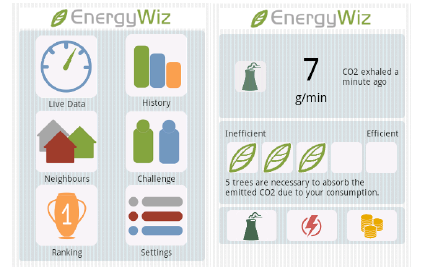
\includegraphics[width=0.7\textwidth]{./Images/energywiz}
\caption{Energy Wiz: main menu and live data}
\label{fig:energywiz}
\end{figure}

\item \textbf{Comparison:} 
comparison has been demonstrated to be an effective strategy in fostering behavioral change. In general terms, there are two types of comparisons: self-comparison (comparison between one’s current and past data) and social (comparing one’s data to that of other households). Social comparison fosters competition \cite{Froehlich2010} and could then strongly motivate behavior change. According to \cite{Petkov2011}, three main types of social comparative feedback can be identified:

    \begin{itemize}
        \item Normative: it consists in the comparison between the user’s data and a reference value / an averaged performance. The main issue with the normative comparison is that users are prone to be suspicious about the validity of the group they are assigned to \cite{Darby2006,Fitzpatrick2009}. 
        \item  One-on-one: as the name suggests, it consists in the comparison between two individuals, and has been demonstrated to be more effective if the two individuals are closely related (e.g. friends) or share the same beliefs and opinions.
        \item Comparison by ranking consists of comparing groups which are ordered depending on their performance. This type of comparison helps to foster a sense  of competitions between individuals or groups that are not closely related.
        
        In \cite{Petkov2011} the effectiveness of self-comparison, normative comparison, one-on-one comparison and ranking is tested. To this aim, the authors developed the EnergyWiz application, which combines the above-mentioned feedback types , is integrated with Facebook, and allows users to share their consumption or challenge other people to save energy. 
    
    \end{itemize}

\item \textbf{Goal Setting:}
goal setting is a powerful source of motivation and, when combined with feedback, is particularly effective in stimulating environmentally responsible behaviors \cite{Froehlich2010}. The Energy Life application \cite{Giulio2009}(\cref{fig:energylife}) largely relies on such game-like rational. The main aim of this project is to increase people knowledge about the impact of their consumption patterns and does so by combining awareness tips and consumption feedback. Energy Life presents the users with a series of goals, as well as tips to reach them, tailored on their own consumption habits. Also, the above-mentioned EnergyWiz app \cite{Petkov2011} presents a similar feature. In order to increase savings and users engagement, EnergyWiz allows users to challenge a Facebook friend of theirs by proposing an energy saving competition. Results from the interviews with the users revealed that this feature was their favorite. 

\begin{figure}[h]
\centering
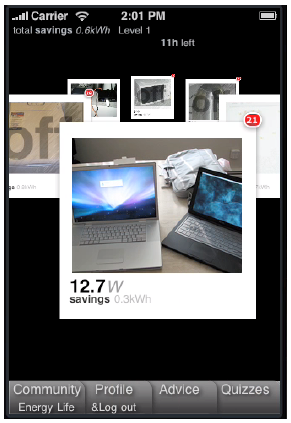
\includegraphics[width=0.3\textwidth]{./Images/energylife}
\caption{Energy Life Menu}
\label{fig:energylife}
\end{figure}

\item \textbf{Commitment:}
it has been widely demonstrated that when a person commits him/herself to behave in a specific way, the probability that s/he will pursue that behavior increases \cite{Froehlich2010}. In the field of \ac{EF}, for instance, public commitment could lead to energy savings of around 20\% \cite{CommitmentandVoluntaryEnergyConservation}

\item \textbf{Incentive / Disincentives and Rewards / Penalties:}
according with Froehlich et al. \cite{Froehlich2010} also incentives/disincentives and rewards/penalties can be used as motivation techniques when designing an \ac{EFS}. Specifically, the former two are antecedent motivation techniques, since they come before a behavior, while rewards and penalties are consequence motivation techniques, which should be used to provide users with some insights into what behaviors they should pursue and what to avoid \cite{Froehlich2010}. Indeed, as pointed out in \cite{Giulio2009}, feedback should not only punish or discourage bad habits but also encourage good ones.

\item \textbf{Frequency and temporal granularity:}
researchers agree that feedback has a positive impact on behavior change. However, it is a way more efficient if given frequently \cite{Feedbackonhouseholdelectricityconsumption:atoolforsavingenergy?}. The real-time feedback is the most effective one \cite{Froehlich2010} since it helps the users making an immediate connection between an action and its impact, thus making the information more relevant for the user \cite{Fitzpatrick2009}. At the same time, the historical detailing of energy consumption is a highly appreciated feature \cite{Giulio2009, Petkov2011} and helps increasing users awareness about their energy patterns \cite{Fitzpatrick2009}.

\item \textbf{Media/device:}
some of the studies \cite{Fitzpatrick2009, Froehlich2010, Pereira2013} also highlight the importance of the mobility aspect. Households usually value the opportunity to access the feedback and check their energy status via mobile devices.

\end{enumerate}

\subsection{Research studies on EFS}

\textbf{\ac{SINAIS} project}


Over 40 years of research on \ac{EF} has yielded many insights into designing and effective \ac{EFS}, nevertheless, there are still some interesting research questions to answer and technological solutions that could be used to improve the effectiveness of such systems. This section presents some of the research studies done in recent years for the purpose of \ac{SINAIS}, a research project developed by researchers from the Madeira Interactive Technologies Institute, where part of the present work has been carried out.


\ac{SINAIS} is a long-term real-world research project that combines \ac{NILM}, social networking and context awareness to understand and motivate people to reduce their energy consumption while trying to fill the lack of research studies that assess the long-term effects of \ac{EFT} \cite{Pereira2012}.


\ac{NILM} - which consists in a system that separates data collected from a single point of measurement into appliance-specific energy consumption data, by using signal processing, and statistical learning - acquires data from sensors that measure current and voltage and then converts them into traditional power metrics. Every time that a significant change in the signal is detected, it is flagged as an event for further processing (i.e. power event are classified through machine learning algorithms). At the end of this process, it is possible to estimate the energy consumption by appliance. One of the main requirement for the study was to develop a low-cost \ac{NILM} solution, which could be deployed in dozens of houses while keeping the installation and monitoring costs low.


 In terms of hardware components, the custom end-to-end \ac{NILM} home energy monitor system developed for the purpose of \ac{SINAIS} consists of a simple netbook. Current and voltage are sampled by using the netbook’s built-in Analog to Digital Converter of the audio input. Feedback on energy consumption is provided through display and speakers, and the communication over the Internet is performed using the Wi-Fi card. In addition, in order to monitor users’ engagement with the system, microphone, and built-in camera were used to sense human-activities.  From the software side, data is read from the sensors using Java sound \ac{API}, and then stored in a centralized repository that uses a web-based hosting service to keep all database files synchronized in one place as long as there was internet connection available. The database is updated every 20 minutes by the meters. The server has many RESTful web-services to access data aggregated in several ways. \Cref{fig:sinais}  illustrates the SINAIS NILM software architecture.
 
 \begin{figure}[h]
\centering
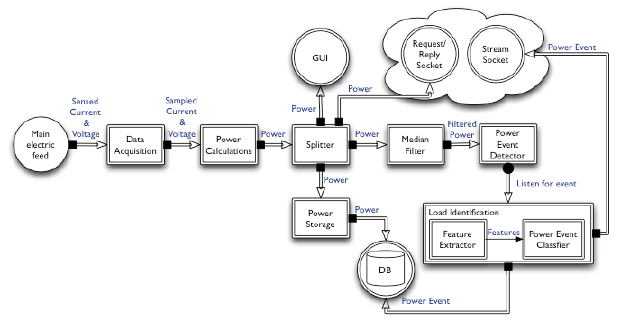
\includegraphics[width=0.8\textwidth]{./Images/sinais}
\caption{\ac{SINAIS} architecture}
\label{fig:sinais}
\end{figure}


As stated above, despite a large amount of research in the area of \ac{EF}, almost all studies are limited to short periods of time, thus resulting in a reduced knowledge of the effectiveness of \ac{EFS} in the long-term. For this reason, as part of \ac{SINAIS}, the \ac{NILM} system previously described was used in a one-year study, precisely aimed at deepening our understanding of long-term effectiveness of \ac{EF} \cite{Pereira2013}. A total of 12 families used the system for 52 weeks. Results show that after about 4 weeks users stopped paying attention to the system, suggesting that \ac{EFS} are not particularly effective in keeping users engaged over time. To test this hypothesis, a new interface (\cref{fig:efs1}) was introduced (week 8), resulting in an immediate increase in the user interaction. Nevertheless, once the novelty effect has passed (three weeks after the introduction of the new \ac{UI}), the number of interactions dropped again. The same phenomenon was observed around week 20 and 42 when the research team conducted some interviews which temporarily raised participants awareness about the system.
At the end of the study, the interactions decrease was of 90\%. When asked about this decrease of interest in the \ac{EFS}, users justified it due to lack of time as well as for result of a more accurate picture of their consumption patterns


\begin{figure}[h]
\centering
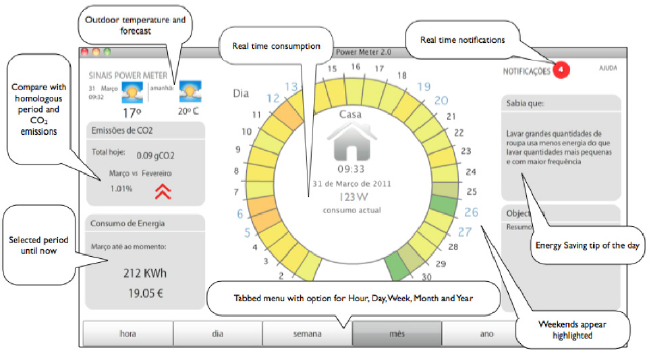
\includegraphics[width=0.8\textwidth]{./Images/efs1}
\caption{The\ac{SINAIS} \ac{EFS} layout}
\label{fig:efs1}
\end{figure}


In order to understand what could lead users to retain attention over time, families’ motivations for sustainable behaviors were further investigated in a two-year study \cite{Barreto2014}.


Interestingly, after interviews with the 15 families that participated in the study, it was found that motivations for sustainable behavior may not be rooted only on individuals’ environmental concerns and/or need for expense management. Other motivations emerged from the study, and not reported in the literature, are:

\begin{enumerate}
    \item parenting: parents’ self-perceived responsibility of their role as parents may lead them at engaging with eco-friendly behaviors;
    \item self and family identity: sustainable behaviors as an expression of a pro-environmental identity;
    \item the sense of control: families reported a need to know more about their consumption pattern as well as its impact. Accessing this information provided them with a sense of control of their actions.
\end{enumerate}

Another aspect that deeply influences people willing to adopt more sustainable behaviors  is related to families routines. Indeed, it was found that families (especially those with young children) are less committed to change their consumption habits if they feel it could compromise or affect the completion of the household’s daily tasks. 


Last but not least, household size and children age (if any) have been found to be key variables in understanding families’ latent motivations for pro-environmental behaviors, suggesting that different family types have different motivations. For instance, routine and parenting seemed to be the main motivations of families with young children, while motivations of parents with older children (older than 10 years old) are mainly rooted in short-term goals, like the need for expense management. To sum up, results from this last study suggested that an EFS able to foster long-lasting behavioral changes must go beyond individual ideals of pro-environmental behavior and address basic family needs.


\subsection{Commercial projects}

Not only the research community is involved in the area of \ac{EF}. Many \acp{EFS} are available on the market. Some of the noteworthy products are presented below.



\textbf{Open Energy Monitor} \cite{HomeEnergy}: \ac{OEM} system monitors in real time the energy consumption/production (solar or electrical) and provides feedback also regarding historic data and energy cost. It is fully open-source (hardware and software). The hardware is Raspberry Pi and Arduino based and works over wifi. Market price ranges from about 155£ (without sensors) to 189.80£   for the solution including all sensors \url{https://shop.openenergymonitor.com/emonPi-3}.


\textbf{Sense} \cite{sense}: consists of a small computer, connected to the electrical panel, that monitors both solar production and energy consumption (overall as well as appliances breakdown). Through an application, it provides feedback about: 
\begin{enumerate}
    \item real-time consumption / production; 
    \item historical energy trends (available by day, week, month and device) and; 
    \item usage statistics for individual appliances.
\end{enumerate}

 This system requires a few weeks of training in order to recognize the devices and does so through advanced machine learning algorithms.The price is higher compared to \ac{OEM} and ranges from 299\$ (for the system monitoring only power use) to 349\$ for “Sense Solar”. Also, the fidelity of the results decreases when the network of sense users is small because machine learning algorithms will produce less reliable results.



\textbf{Efergy} \cite{efergy}:
claims 25\% savings in the electricity bill (more than the 10-15\% reported in \ac{EFS} literature), but no data or studies to prove that were found. Their Online Energy Monitor Home \& Solar consists of a real-time energy monitoring system that can be integrated with a set of smart-plugs and a mobile app to monitor and control the single appliances. This system is powerful but not easy to install and also quite intrusive since it requires installing a socket for each appliance to control. As an example, a complete kit with five meters has a cost of 219,60€\footnote{This value was consulted in September 2018: \url{https://efergy.com/store/en/online-energy-monitors/18-online-multi-circuit-energy-monitoring-kit.html\#/35-number_of_circuits_to_monitor-5_x_1ph_circuit}}, and extra meters are about 54,90€\footnote{This value was consulted in September 2018: \url{https://efergy.com/store/en/accessories/22-submetering-kit-stxtra.html\#/28-select_your_power_supply-3_phase_up_to_90a_phase}}.



\textbf{Neurio} \cite{neurio}: is another monitoring system that can be easily installed within the home’s load panel and provides feedback on both production and consumption.



\textbf{Energeno}: developed several models of energy monitoring systems. Despite these systems were pretty well-known and have been analyzed in several research studies, Energeno has ceased trading.


\subsection{Conclusions}

The projects listed above combine many \ac{EF} techniques like real-time feedback, which is one of the most effective \cite{Froehlich2010}. The \ac{SINAIS} project introduced machine learning algorithms to identify the source of energy consumption, however, despite users appreciated the opportunity to better understand what appliances consume more \cite{Pereira2013}, after one year deployment, the decrease of energy usage was not significant. This result supports the hypothesis that \acp{EFS} are not effective in the long term because, as suggested by results from \ac{SINAIS}, after a while people lose interest in the system which becomes “just another electric device” \cite{Pereira2013}. Another important lesson learned is that \acp{EFS} must be designed to adapt to different users (and, consequently, different behaviors, needs, and interests). For the same reason, as demonstrated in several of the studies reviewed, the mobility aspect is extremely important. Users want indeed to access their data quickly and from virtually everywhere; that’s why commercial \acp{EFS} like Sense and Efergy provide users also with a mobile application. Ultimately, it is important to point out two main weaknesses of \acp{EFS}. On the one hand, the cost. \acp{EFS} available on the market are quite expensive and this could explain their low adoption rate. On the other hand, the fact that their effectiveness decrease in the long-term \cite{Pereira2013}, which suggests the need for thinking about solutions that could keep users engaged and interested in the system over time. 



% #############################################################################
\section{Energy Trading Systems using blockchain} \label{sets}
\subsection{Blockchain}

The blockchain is a technology for peer-to-peer platforms that have a decentralized storage to record all transaction data. This technology came into the public in 2008  when a publication by Satoshi Nakamoto (a pseudonym for the creators) was launched Bitcoin, describing it as a \ac{P2P} electronic cash system that enables online payments to be transferred directly without an intermediary \cite{bitcoin}. Bitcoin is one application of the blockchain concept, the first and the most known one:  “Blockchain is to Bitcoin, what the internet is to email. A big electronic system, on top of which you can build applications. Currency is just one.” - Sally Davies, FT Technology Reporter \cite{Howbitcoinanditsblockchainwork}. However, this technology has great potential in many sectors, not only in the financial one.


First, we will introduce the main concepts before explaining how they will be applied in this project. The blockchain concept relies on the decentralization idea. A decentralized storage and decentralized business without the need of a trusted third party are the base of this technology. A short time ago, all money transactions were executed by trusted third parties like banks and governments, resulting in extra costs for the customers. The role of those entities is to authenticate both participants of the transaction (the emissary and the receptor) and keep the record as a confirmation of the transaction. In this digital world, it is even more important to securely store the record of the transactions in order to prevent any malicious activities. 



\subsubsection{Overview}


Electronic coins are chains of digital signatures and a transfer is done signing a hash of a previous transaction and the public key of the next owner and finally adding these to the end of the chain \cite{bitcoin}. The main problem here is a guarantee that the coin is not double-spended \footnote{the ​double spending problem ​is a potential flaw in a cryptocurrency or other digital cash scheme whereby the same single digital token can be spent more than once, and this is possible because a digital token consists of a digital file that can be duplicated or falsified.Chohan, Usman, The Double Spending Problem and Cryptocurrencies (December 19, 2017). Available at SSRN: \url{https://ssrn.com/abstract=3090174} or url{http://dx.doi.org/10.2139/ssrn.3090174}}. Usually, the double-spend problem is solved by a centralized trusted authority that is responsible to guarantee that the rules are not broken. This is a single point of failure approach, \textit{technically speaking} this means that the centralized authority has all data (electronic coin representation) in the same place (or machine) and in case of this data be compromised, all the system will be compromised too, in the trusting level, the users of a system with this approach are required to trust in the authority and if that authority is a malefactor all the user data will be in risk.  The blockchain technology eliminates the need for intermediaries, validating the transactions in a decentralized way. 


The transactions are carried out between peers who can be providers, consumers or both. The data that contains all the relevant information about the transaction is stored on a distributed ledger and all peers store the block of data locally. A distributed ledger is a distributed database that records, shares and synchronizes transactions in different locations. It is efficient, resilient and reliable. 


Ideally, all of the transactions have a smart contract behind. Smart contracts define the rules related to the transaction, like a transactions protocol that executes the terms of a contract \cite{SmartContracts}. \cref{fig:bc} demonstrates the idea of transaction validation.



 \begin{figure}[h]
\centering
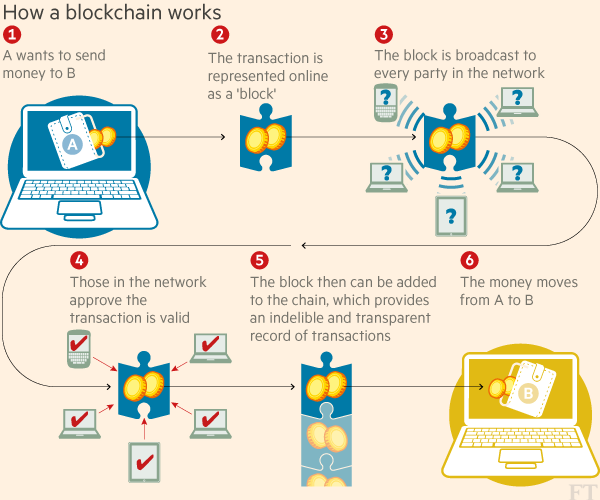
\includegraphics[width=0.8\textwidth]{./Images/ft}
\caption{Illustration about transaction validations workflow in blockchain}
\label{fig:bc}
\end{figure}


Each transaction is encrypted and distributed to individual computers and each member of the network stores the data locally. Each block is verified using hash algorithms and associated with a hash that is unique and is related to the information on the blockchain. If the information on the block is changed after the transaction, the peers cannot verify the block because the correct hash is not produced anymore, and the block is discarded.



The continuous verification is called mining and is performed by the members of the network. The mining is necessary to ensure that everyone agrees on the order of the transactions. Each block is like a package of transactions and is associated with a timestamp, a nonce and a reference to a previous block (i.e. the hash of the previous block) \cite{bitcoin}. All these blocks connected form a blockchain that is constantly growing and represents the state of the ledger.


To establish that consensus, both proof-of-work and proof-of-stake are used.
In the \textbf{proof-of-work} approach, each block is verified by a large group of peers before storage using algorithms that associate a unique hash (ordinary or cryptographic) to the block. The verifying task is very complex because it is necessary to find a hash that corresponds to the block content. The block cannot be changed without re-doing the work and if a new block is added to the chain after this one, all blocks after this need to also re-do the work \cite{bitcoin}. This process requires a lot of energy. If the majority of peers verifies a block content it can be added to the blockchain, otherwise, it is discarded. This majority decision is represented by the longest chain, which means the one with the greatest proof-of-work effort invested \cite{bitcoin}. 


\textbf{Proof-of-stake} approach is simpler than the proof-of-work approach because it requires that users prove ownership of their own share (stake). So, if a user owns 10\% of total data he just needs to be mining 10\%. This reduces the complexity of the task and is less expensive in terms of costs and energy consumption \cite{etherium}.
Summarizing, the steps performed in a blockchain network are \cite{bitcoin}: 

\begin{enumerate}
    \item New transactions are broadcasted to all nodes. 
    \item Each node collects new transactions into a block. 
    \item Each node works on finding a difficult proof-of-work for its block. 
    \item When a node finds a proof-of-work, it broadcasts the block to all nodes. 
    \item Nodes accept the block only if all transactions in it are valid and not already spent. 
    \item Nodes express their acceptance of the block by working on creating the next block in the chain, using the hash of the accepted block as the previous hash.
\end{enumerate}


The main disadvantage of the blockchain technology is its performance. The blockchain technology implies heavy calculations, the mining process explained above, to generate and verify the signature of each block. Due to its decentralized nature, an extra effort is necessary to ensure a consensus exists in the network. Consequently, the total amount of computation that a blockchain requires per node in the network is very expensive in relation to a centralized database. The fact that blockchain is a recent technology can be seen as disadvantageous because it is necessary for a new technology to have existed for a longer period of time in order to increase cultural adoption and trustworthiness. The large energy consumption in Bitcoin blockchain is a very big problem, but this problem was reduced with the emergence of the Etherium approach which uses three times less energy than Bitcoin because it uses the proof-of-stake method to verify transactions.


The advantages of the blockchain technology are bigger than the disadvantages. The main advantages include lower costs, faster processes and greater flexibility because no more third parties are needed and no central point of failure exists once the storage and communication are fully decentralized. All the time and money spent to prevent tampering in centralized databases is not necessary anymore, because in blockchain the storage is not centralized. Other significant advantages are the control that users can have over all the information and transactions, the consistency and availability of the data, the trustworthy process of each transaction, the faster transactions and the lower costs per transaction.


\subsubsection{Integration in the energy sector}

Traditionally, the Electrical Power Systems are controlled via a top-down approach where central authorities are responsible to manage the energy distribution in the grid. Lately, new decentralized approaches are being investigated in order to create a full transparency and to allow micro producers and consumers to reap the full economic benefit of the energy sharing system without the participation of central authorities. The Blockchain could be applied to the energy market providing a secure decentralized network to share energy \cite{Hasse2016}. There is an especially high potential for \ac{ET}, automation of processes and new business models \cite{UseCasesforBlockchainTechnologyinEnergyCommodityTrading}. Another novel application is the use of cryptocurrencies in the payment system. The storage of energy data can also be re-designed to work over blockchain technology with smart contracts and verification of transactions ensuring the integrity of the data and trust between the grid participants \cite{ETHome:Opensourceblockchainbasedenergycommunitycontroller}. For example, in a smart grid, a producer who has more energy than he needs can automatically sell the excess energy via a smart contract to neighbours who want to buy energy. This example can be done in the reverse order, i.e. consumers can automatically buy energy from other producers.


 The concept of a blockchain based distributed controller for the efficient share of \acp{ESS}  has been proved showing that the concept is applicable, scalable and economically feasible \cite{ETHome:Opensourceblockchainbasedenergycommunitycontroller}. Also, secure and privacy-friendly protocols were designed for trading and billing in Smart Grids \cite{SecureandPrivacy-FriendlyLocalElectricityTradingandBillinginSmartGrid} and can be applied. 

\subsubsection{IOTA and the Tangle}
\label{seciotatech}


Since increasing the consumption of renewable energy is one of the main goals of the present work, it would have been inconsistent to not use an efficient blockchain platform. After some research, the IOTA distribution ledger technology has been identified as the most suitable solution for that purpose. IOTA is an open-source distributed ledger, which differs from blockchain concepts like Bitcoin or Ethereum, since it uses “The Tangle”, a \ac{DAG} characterized by high scalability and low resource requirements. The Tangle eliminates one of the biggest drawbacks of blockchain, that is to say, it removes fees \cite{WhatisIOTA}. Since IOTA cryptocurrency is open source and blockless, users can make transactions on the network for free. In addition, this cryptocurrency is very well rated in terms of market capital (10th place, at the time of this writing \url{https://coinmarketcap.com/}).  The absence of fees is extremely important, especially when we are talking about micropayments, like in the case of \ac{P2P} \ac{ET}. While in traditional blockchain transactions are grouped into blocks and stored in sequential chains, the Tangle is blockless and no third party is needed. Individual transactions are interconnected in a \ac{DAG}. For example, let’s take a scenario where A, B, C and D are different nodes of the network, and A wants to communicate with D. In a traditional blockchain network, which is sequential, the transaction between A and D needs to be distributed and validated by both B and C before it gets to D. On the contrary, on the Tangle A, B, C, and D are connected in a braid-like fashion, thus, when A needs to communicate with D, it sends the data directly to D while synchronizing (almost) instantaneously B and C. Consequently, the energy spent for the proof-of-work is reduced, since consensus is established only by the participants making transactions instead of miners.


The main idea of the Tangle is that, when a transaction issued by a node arrives, it must approve at least two previous transactions. This way, users who issue a transaction are also contributing to the security of the network \cite{TheTangle}. Steps to issue a transaction are the following \cite{TheTangle}:

\begin{itemize}
    \item Signing the transaction with private keys;
    \item Selecting two “tips” (i.e. unverified transactions) using \ac{MCMC}) algorithm. Then, if they are not conflicting, the node approves them;
    \item Solving a cryptographic puzzle by finding a nonce such that the hash of that nonce concatenated with some data from the approved transaction has a particular form.
\end{itemize}

After a transaction is performed, it is broadcasted in the network and validated by the active members of that network. To keep the state of the network a consensus protocol is used, which decides if a transaction could be safely considered confirmed or not. 

The \cref{fig:tangle} below represents the structure of the Tangle and how the validation process works - green nodes are the verified transactions; red nodes represent transactions in process of verification; grey nodes are the unverified transactions (tips).
Green blocks are indirectly referred by all the grey blocks, thus, for every confirmed transaction there is a path that goes to a tip. Now, the node runs the tip selection algorithm (\ac{MCMC}) N times; the number of times the transaction is selected determines the confirmation level of that transaction. For instance, if a transaction is selected 55 times during 100 runs of the \ac{MCMC} algorithm, that transaction is confirmed with 55\% confidence.



 \begin{figure}[h]
\centering
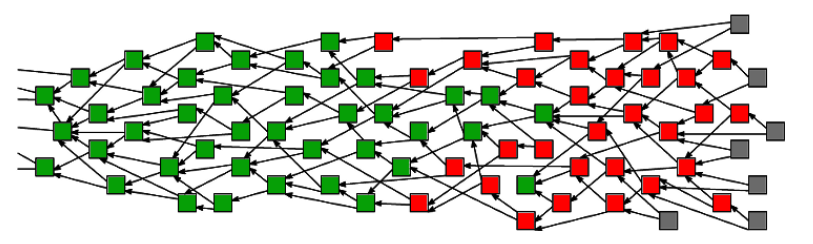
\includegraphics[width=0.8\textwidth]{./Images/tangle}
\caption{The thangle \ac{DAG}}
\label{fig:tangle}
\end{figure}


To sum up, the main features of IOTA are:
\begin{itemize}
    \item Data Transfer through the tangle in a secure and authenticated way.
    \item Masked Messaging: all the exchanged data can be encrypted and authenticated. With \ac{MAM} data is shared by multiple parties and these multiple parties can adjust the frequency and get the broadcast data.
    \item Everything as a service: anything with a chip can be leased in real time.
    \item Scalable ledger.
\end{itemize}


In order to perform transactions on the Tangle, users need to have an IOTA seed, which consists of an 81, 162 or 243 characters string (only uppercase Latin letters and 9’s) and is generated randomly. Through the seed, a user can access his/her IOTA account, thus, the seed is secret and must be securely stored. In addition, to receive payments, the user needs a destination address. This address is generated from the seed and can be public.


Further details about how the Tangle works and how it will be employed in this project are provided in \ref{ii} \nameref{ii}. 


\subsection{Research projects and startups}
\label{rps}


At the time of this writing, several projects have been launched with the goal of building a distributed energy system. According to the Event Horizon 2018 Startups report, about 41 startups are developing blockchain-based energy applications (25 of them in Europe), nevertheless, after a quick search, a lot more blockchain startups working in the energy field can be found \cite{EnergyBlockchainStartups}. In this scenario, Etherium seems to be the most used blockchain protocol \cite{STARTUPSWHOISWHO}.



Below, a review of some existing projects is provided. Given the rapid evolution of this sector, such review makes no claim to be comprehensive. In addition, the reader should be warned that most of the projects here described are under development, thus many details about them are still unknown. 



\textbf{Electron} has been launched by “a team of blockchain, energy and e-trading professionals using decentralized technology to advance the shared infrastructure of the energy markets” \cite{Electron}. In general terms, Electron is a marketplace for energy and flexibility services underpinned by a \ac{DER} asset registry \cite{STARTUPSWHOISWHO}.
Their approach is more collaborative, top-down than peer-to-peer. Electron is looking for a shared infrastructure and collaboration opportunities to change the energy market. One of the main projects they are involved in aims to unlock \ac{DSR} by using blockchain technology \cite{demand-sideresponse}. The goal of this project is creating an incentive for everyone in the market (grid operators and large energy users); users that reduce their energy consumption on peak periods will receive a payment for that and consequently if the demand is reduced at peak time the electricity prices should lower.



\textbf{Power Ledger} is a decentralized \ac{ET} blockchain based platform that enables residential and commercial businesses connected to the existing distribution network to decide to whom they sell their energy and at what price \cite{STARTUPSWHOISWHO}. Their solution is peer-to-peer and allows direct selling and buying between micro producers and consumers without a third party involved and with payment in real time. The system is based on blockchain but the payments are made with fiat-currency\footnote{is a legal tender that is backed by the sovereign government state that issues it. The
Australian dollar and U.S. dollar is fiat money, as are many other major world currencies. This differs
from money whose value is underpinned by some physical good such as gold or silver (commodity
money).}.



Power Ledger is a dual-token platform: POWR tokens are used to access the platform and can be exchanged for the other token (Sparkz), which is stable (i.e. pegged to fiat currency) exchangeable frictionless \ac{ET} token Spark must be pre-purchased \cite{powerledgerwhitepaper} and can be then redeemed for fiat currency. \cref{fig:plp2p} represents the \ac{P2P} trading between consumers and prosumers through Power Ledger. 




 \begin{figure}[h]
\centering
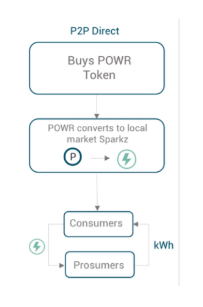
\includegraphics[width=0.3\textwidth]{./Images/plp2p}
\caption{\ac{P2P} trading through Power Ledger}
\label{fig:plp2p}
\end{figure}


To sum up, users must buy POWR tokens to sign in and use the platform. After that, POWR tokens are converted to Sparkz (local market level token), which in turn can be used to perform the frictionless exchanges - that is to say, payments for the transactions are made via local currency, not cryptocurrencies. Power Ledger has adopted a hybrid public and consortium blockchain approach. POWR tokens are generated on the public Ethereum blockchain (proof-of-work algorithm), while for the P2P \ac{ET} a fee-less Ethereum blockchain is used. The next step is migrating all system on a public proof-of-stake blockchain, which would be more sustainable. Specifically, this blockchain is called EcoChain and is still under development.



So far, Power Ledger is one of the most advanced projects in this area and has been successfully pilot-tested since 2016. The first pilot was indeed a big success; 15 dwellings were connected via blockchain, so to provide them with a secure channel for direct exchange between Sparkz and currencies in real-time, and used distributed ledger technology to facilitate “across the meter” \ac{ET} and manage the \ac{DER} assets without going through an electricity retailer. Power Ledger algorithm is developed to respond in real-time to both network conditions and consumer behavior.   


\textbf{LO3 energy Inc.} is developing blockchain based solutions for the energy market \cite{lo3energy}. Together with \textbf{Transactive Grid}, LO3 designed the first community-powered microgrid: the \textbf{Brooklyn Microgrid} \cite{lo3energy}. Using blockchain, residents with solar panels can sell excess energy to their neighbours in a peer-to-peer transaction.The energy is transmitted by the conventional power grid, and transactions are recorded d and managed using the EXERGY, a blockchain enabled platform with smart contract functionality at its core [source]. Production and consumption data are collected through smart meters and then hashed into the blockchain. Through a mobile app, users can also choose what to do with their excess energy(i.e. storing it into the battery, or selling it to the grid or to the neighbors (figure xx, 4th image).  The Brooklyn Microgrid A \cref{fig:microgrid}, rated 4.9 out of 5 on Google Play an App Store, presents the following main features:

\begin{itemize}
    \item Check out the solar panels locations and suggest new ones;
    \item Check solar panel efficiency and where leftover energy is going;
    \item Energy usage feedback (up to 12 months).
\end{itemize}

\begin{figure}[h]
\centering
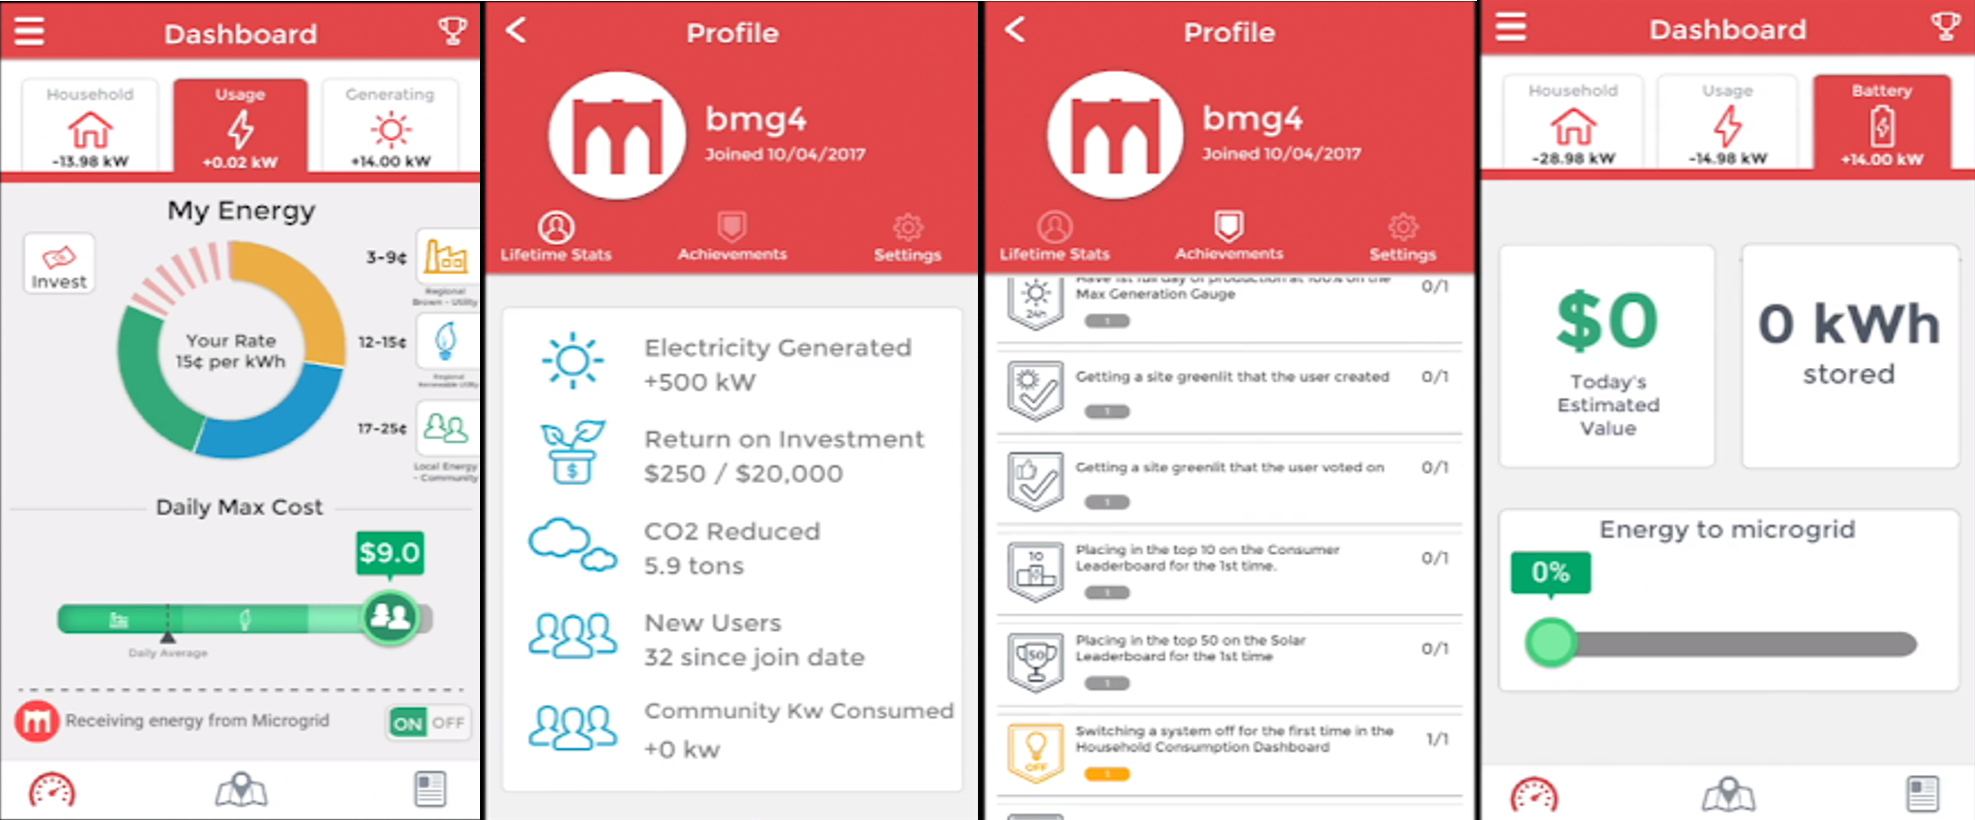
\includegraphics[width=0.9\textwidth]{./Images/microgrid}
\caption{Brooklyn Microgrid application layouts}
\label{fig:microgrid}
\end{figure}

The App works as follows. First of all, users have to set how much are willing to pay for their energy a day (see \cref{fig:microgrid}, 1st image). Such value will consequently determine the source of the energy users are buying. Price of locally generated energy is driven by the participants in the local network \cite{vimeo}. In addition, users are provided with the opportunity to turn off their appliances in case of grid overload and get paid for that. Users’ energy stats is provided in the profile page (see \cref{fig:microgrid}, 2nd image). Last but not least, in the achievements sections, users can showcase their reputation as advocates for local energy (see \cref{fig:microgrid}, 3rd image).



\textbf{Omega Grid} consists of a private cyber secure distribution market \cite{STARTUPSWHOISWHO} which uses a blockchain based Financial Energy Resource Management System  to record communications, verify power delivery, and perform transactions. The communication is done via a private mesh network. Omega Grid connects local distribution companies with both prosumers and consumers, providing benefits for all of them \cite{omegagrid}. Like Power Ledgers and Brooklyn microgrid, Omega Grid effectively transmits energy through local grids. Omega Grid uses an energy efficient Proof of Authority consensus model (basically, an optimized Proof of Stake model) that use identity as a form of stake instead of  staking tokens. A group of pre-approved validators is then responsible for staking the identity \cite{poa}. 




\textbf{Leap} is a platform that enables automated trading on energy markets for anyone, including aggregators, utilities and \acp{ISO}.


The platform is based on the \ac{DEX}, which basically consists in an open energy market that allows for fully automated trading of energy resources \cite{leap} (see \cref{fig:leap}). The main goal of Leap is reducing power consumption in peak hours. For this purpose, the \ac{DEX} collects  information about load reduction rewards programs from \acp{ISO} and utilities.


\begin{figure}[h]
\centering
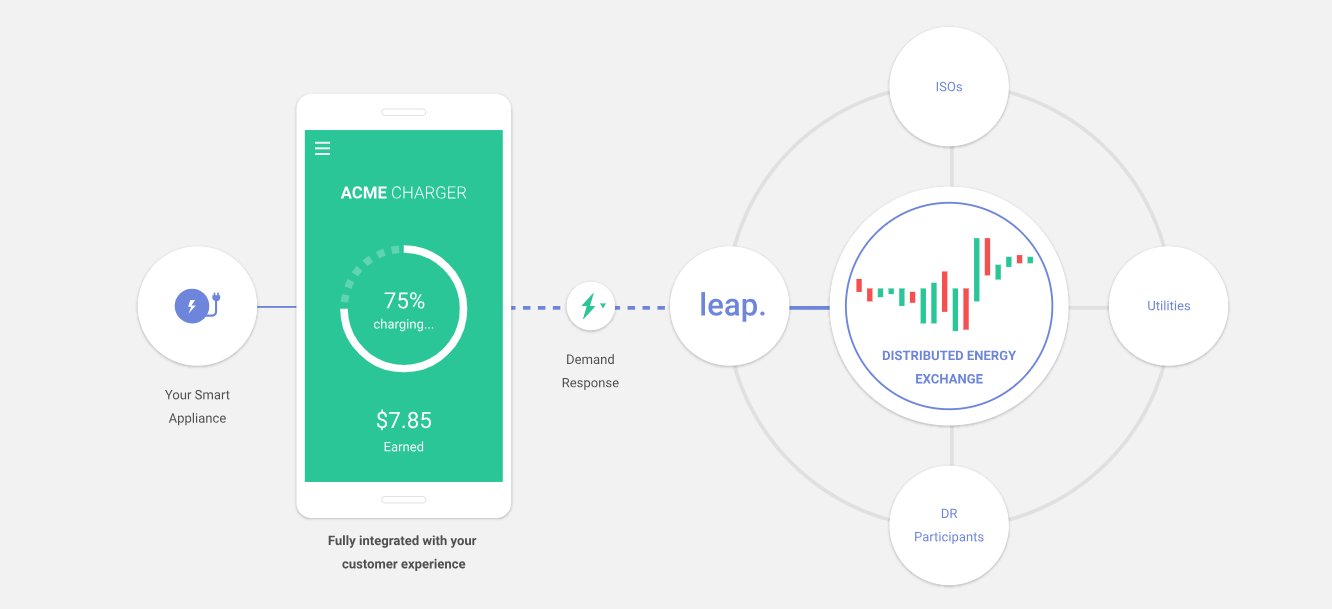
\includegraphics[width=0.8\textwidth]{./Images/leap}
\caption{Leap overview}
\label{fig:leap}
\end{figure}

Then, on the basis of smart contracts, it performs Demand Response control and sends meter data back to the \acp{ISO}, who verifies load reduction and remits funds to accordingly. 


\textbf{Grid Singularity}, a startup based in Australia, is developing an open and decentralized energy data exchange platform. The core of the platform is DA3,  a grid management agent that creates a novel market model for the transactive grid, enabling a wide spectrum of energy market-related transactions on a single platform layer via blockchain. The platform will be launched in 2019 thus many details are still unknown. Nevertheless, according to an interview to the CEO of Grid Singularity, Ewald Hesse, the platform will work as follows:
\textit{“All data will be recorded in real time on the blockchain, what will make it fully secure and impossible to modify. Once the platform is ready, it will be able to support numerous applications, for example for data analysis and benchmarking, green certificates, smart grid management, investment decision, and energy trade validation. The core product will be invisible for the end users – all that they’ll have to do is download an app that will make their houses single traders in the market”}\cite{gridsingularity}.  	



It’s impossible to list all the projects that are being developed in this field since their number is growing almost on a daily basis. \textbf{Enerchain}, for example, is another blockchain based distributed ledger for energy tradings that use Tendermint\footnote{Tendermint is software for securely and consistently replicating an application on many machines. Works even if up to 1/3 of machines fail in arbitrary ways. Every non-faulty machine sees the same transaction log and computes the same state.See more:\url{https://tendermint.readthedocs.io/en/master/introduction.html}
} technology to guarantee a short block time in order to allow tradings almost in real-time \cite{enerchain}. \textbf{Powerpeers} developed a similar system for P2P \ac{ET}, not based on blockchain yet, that is currently being deployed in Amsterdam \cite{powerpeers}. 



\textbf{\ac{EWF}} is an open-source, scalable, blockchain platform designed for the energy sector. The vision of \ac{EWF} is joining forces to accelerate the transaction to a decentralized, democratized, decarbonized, and resilient energy system. 
	
	
	
Except for Brooklin Microgrid and Grid Singularity, all the projects here described uses Ethereum blockchain. Brooklyn Microgrid uses Exergy and Grid Singularity uses Energy Web Chain.


The author considers using Etherium as a disadvantage since Ethereum transactions have fees (to “cover” the computing power needed for the proof-of-work). To overcome this issue, Power Ledger, for instance, has developed the EcoChain, a more sustainable blockchain, while Omega Grid uses proof-of-authority consensus model instead of proof-of-work.



Electron, Omega Grid, and Power Peers act like an intermediary between energy suppliers and all possible consumers. It is also important to notice that many of the projects and startups described above still need to be deployed and pilot tested. At the time of this writing, only Brooklyn Microgrid, Power Peers and Omega Grid have successfully reach the market. Power Ledger project is well documented and a lot of experiments have been done so far to test the platform. Nevertheless, it has not been launched to the public yet, so it is hard to evaluate it.



Last but not least, it should be pointed out that only Power Peers, Power Ledger and Brooklyn Microgrid have as main target micro producers and consumers. Focusing on the local community first is a promising strategy since each community has its own cultural attitudes and motivations toward engaging in \ac{P2P} \ac{ET}, which should be taken into account when designing such systems. This can be considered an advantage because all the markets have specifics constraints like grid stability, infrastructures architecture and also the cultural differences in the user’s behavior. On the contrary, platforms like Electron, Leap and Omega Grid focus on using blockchain to target energy market problems, like \ac{DSR}, thus opening up space for retailers and electricity companies.   
